\documentclass[../synthesis.tex]{subfiles}
\graphicspath{{\subfix{../../../../images/}}}
\begin{document}
    The \textbf{solid-state reaction}\cite{b9} method is a commonly used technique for the synthesis of various materials, 
    including nanophosphors. It involves the direct reaction between solid precursor materials to form the 
    desired product.The solid-state reaction method offers simplicity, versatility, and the ability to control 
    the reaction conditions for the synthesis of nanophosphors. However, it may require high temperatures and 
    longer reaction times to ensure complete reaction and achieve the desired crystallinity. Optimization of the 
    heat treatment parameters is crucial to obtain nanophosphors with the desired properties and luminescent 
    behavior for thermoluminescence dosimetry applications. Here is an overview of the solid-state reaction method:

    \begin{Figure}
        \centering
        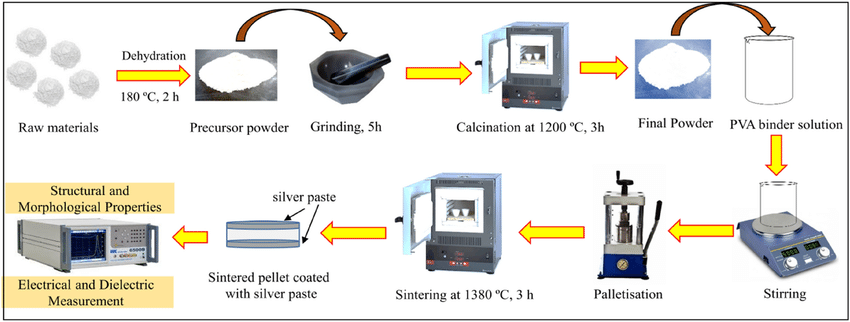
\includegraphics[width=0.8\linewidth]{SolidStateFlow.png}
        \captionof{figure}{Synthesis using Solid State Reaction Method\cite{a9}}\label{fig:SolidStateFlow}
    \end{Figure}
    \begin{itemize}
        \item \textbf{Selection of Precursor Materials: } Choose solid precursor materials that contain the 
        necessary elements for the composition of the nanophosphor. These precursors may be in the form of 
        powders or solid compounds.
        \item \textbf{Weighing and Mixing: } Accurately weigh and mix the precursor materials in the desired 
        stoichiometric ratio. The mixing can be done using mortar and pestle, ball milling, or other mechanical 
        methods to ensure a homogenous mixture.
        \item \textbf{Grinding and Milling: }If the precursor materials are not already in the form of fine 
        powders, grinding and milling steps may be required to reduce their particle size and improve their 
        reactivity. This step facilitates intimate contact and diffusion of the reactants during the subsequent 
        heat treatment.
        \item \textbf{Pelletization or Pressing: }Depending on the application and desired final form of the 
        nanophosphor, the mixture of precursor powders may be pressed into pellets or compacted using a hydraulic 
        press to obtain a solid compact.
        \item \textbf{Heat Treatment (Calcination): }The compacted precursor mixture is subjected to heat 
        treatment in a furnace. The temperature and duration of the heat treatment are critical to promote the 
        desired chemical reactions and facilitate the formation of the nanophosphor phase. The heat treatment 
        process is often referred to as calcination.
        \item \textbf{Cooling and Grinding: }After the heat treatment, the sample is allowed to cool to room 
        temperature. It is then ground or milled again to break up any agglomerates and obtain a fine powder of 
        the nanophosphor.
    \end{itemize}
\end{document}





